\documentclass[11pt,compress,t,notes=noshow, xcolor=table]{beamer}
\usepackage[]{graphicx}\usepackage[]{color}
% maxwidth is the original width if it is less than linewidth
% otherwise use linewidth (to make sure the graphics do not exceed the margin)
\makeatletter
\def\maxwidth{ %
  \ifdim\Gin@nat@width>\linewidth
    \linewidth
  \else
    \Gin@nat@width
  \fi
}
\makeatother

\newcommand{\citebutton}[2]{%
\beamergotobutton{\href{#2}{#1}}%
}

\newcommand{\blu}[1]{\textcolor{blue}{#1}}
\newcommand{\org}[1]{\textcolor{orange}{#1}}
\newcommand{\ques}{\textbf{\textcolor{red}{Question:  }}}
\newcommand{\questionssofar}{\begin{frame}\frametitle{Any questions?}\end{frame}}

\newcommand\warning{%
 \makebox[1.4em][c]{%
 \makebox[0pt][c]{\raisebox{.1em}{\scriptsize!}}%
 \makebox[0pt][c]{\color{red}\normalsize$\bigtriangleup$}}}%

\definecolor{fgcolor}{rgb}{0.345, 0.345, 0.345}
\newcommand{\hlnum}[1]{\textcolor[rgb]{0.686,0.059,0.569}{#1}}%
\newcommand{\hlstr}[1]{\textcolor[rgb]{0.192,0.494,0.8}{#1}}%
\newcommand{\hlcom}[1]{\textcolor[rgb]{0.678,0.584,0.686}{\textit{#1}}}%
\newcommand{\hlopt}[1]{\textcolor[rgb]{0,0,0}{#1}}%
\newcommand{\hlstd}[1]{\textcolor[rgb]{0.345,0.345,0.345}{#1}}%
\newcommand{\hlkwa}[1]{\textcolor[rgb]{0.161,0.373,0.58}{\textbf{#1}}}%
\newcommand{\hlkwb}[1]{\textcolor[rgb]{0.69,0.353,0.396}{#1}}%
\newcommand{\hlkwc}[1]{\textcolor[rgb]{0.333,0.667,0.333}{#1}}%
\newcommand{\hlkwd}[1]{\textcolor[rgb]{0.737,0.353,0.396}{\textbf{#1}}}%
\let\hlipl\hlkwb

\usepackage{framed}
\makeatletter
\newenvironment{kframe}{%
 \def\at@end@of@kframe{}%
 \ifinner\ifhmode%
  \def\at@end@of@kframe{\end{minipage}}%
  \begin{minipage}{\columnwidth}%
 \fi\fi%
 \def\FrameCommand##1{\hskip\@totalleftmargin \hskip-\fboxsep
 \colorbox{shadecolor}{##1}\hskip-\fboxsep
     % There is no \\@totalrightmargin, so:
     \hskip-\linewidth \hskip-\@totalleftmargin \hskip\columnwidth}%
 \MakeFramed {\advance\hsize-\width
   \@totalleftmargin\z@ \linewidth\hsize
   \@setminipage}}%
 {\par\unskip\endMakeFramed%
 \at@end@of@kframe}
\makeatother

\definecolor{shadecolor}{rgb}{.97, .97, .97}
\definecolor{messagecolor}{rgb}{0, 0, 0}
\definecolor{warningcolor}{rgb}{1, 0, 1}
\definecolor{errorcolor}{rgb}{1, 0, 0}
\newenvironment{knitrout}{}{} % an empty environment to be redefined in TeX

\usepackage{alltt}
\newcommand{\SweaveOpts}[1]{}  % do not interfere with LaTeX
\newcommand{\SweaveInput}[1]{} % because they are not real TeX commands
\newcommand{\Sexpr}[1]{}       % will only be parsed by R
\newcommand{\xmark}{\ding{55}}%


\usepackage[english]{babel}
\usepackage[utf8]{inputenc}

\usepackage{dsfont}
\usepackage{verbatim}
\usepackage{amsmath}
\usepackage{amsfonts}
\usepackage{amssymb}
\usepackage{bm}
\usepackage{csquotes}
\usepackage{multirow}
\usepackage{longtable}
\usepackage{booktabs}
\usepackage{enumerate}
\usepackage[absolute,overlay]{textpos}
\usepackage{psfrag}
\usepackage{algorithm}
\usepackage{algpseudocode}
\usepackage{eqnarray}
\usepackage{arydshln}
\usepackage{tabularx}
\usepackage{placeins}
\usepackage{tikz}
\usepackage{setspace}
\usepackage{colortbl}
\usepackage{mathtools}
\usepackage{wrapfig}
\usepackage{bm}
\usepackage{amsmath}
\usepackage{pifont}

\usetikzlibrary{shapes.multipart,shapes,arrows,automata,positioning,calc,chains,trees, shadows}
\tikzset{
  %Define standard arrow tip
  >=stealth',
  %Define style for boxes
  punkt/.style={
    rectangle,
    rounded corners,
    draw=black, very thick,
    text width=6.5em,
    minimum height=2em,
    text centered},
  % Define arrow style
  pil/.style={
    ->,
    thick,
    shorten <=2pt,
    shorten >=2pt,}
}

\tikzstyle{vec}=[draw, rectangle, fill = white, minimum width=5mm, minimum height=1cm, inner sep = 2pt]

\usepackage{subfig}

% Defines macros and environments
\usepackage{../../style/lmu-lecture}


\let\code=\texttt
\let\proglang=\textsf

\setkeys{Gin}{width=0.9\textwidth}

\setbeamertemplate{frametitle}{\expandafter\uppercase\expandafter\insertframetitle}

\usepackage{bbm}
% basic latex stuff
\newcommand{\pkg}[1]{{\fontseries{b}\selectfont #1}} %fontstyle for R packages
\newcommand{\lz}{\vspace{0.5cm}} %vertical space
\newcommand{\dlz}{\vspace{1cm}} %double vertical space
\newcommand{\oneliner}[1] % Oneliner for important statements
{\begin{block}{}\begin{center}\begin{Large}#1\end{Large}\end{center}\end{block}}


%new environments
\newenvironment{vbframe}  %frame with breaks and verbatim
{
 \begin{frame}[containsverbatim,allowframebreaks]
}
{
\end{frame}
}

\newenvironment{vframe}  %frame with verbatim without breaks (to avoid numbering one slided frames)
{
 \begin{frame}[containsverbatim]
}
{
\end{frame}
}

\newenvironment{blocki}[1]   % itemize block
{
 \begin{block}{#1}\begin{itemize}
}
{
\end{itemize}\end{block}
}

\newenvironment{fragileframe}[2]{  %fragile frame with framebreaks
\begin{frame}[allowframebreaks, fragile, environment = fragileframe]
\frametitle{#1}
#2}
{\end{frame}}


\newcommand{\myframe}[2]{  %short for frame with framebreaks
\begin{frame}[allowframebreaks]
\frametitle{#1}
#2
\end{frame}}

\newcommand{\remark}[1]{
  \textbf{Remark:} #1
}


\newenvironment{deleteframe}
{
\begingroup
\usebackgroundtemplate{
\includegraphics[width=\paperwidth,height=\paperheight]{../style/color/red.png}}
 \begin{frame}
}
{
\end{frame}
\endgroup
}
\newenvironment{simplifyframe}
{
\begingroup
\usebackgroundtemplate{
\includegraphics[width=\paperwidth,height=\paperheight]{../style/color/yellow.png}}
 \begin{frame}
}
{
\end{frame}
\endgroup
}\newenvironment{draftframe}
{
\begingroup
\usebackgroundtemplate{
\includegraphics[width=\paperwidth,height=\paperheight]{../style/color/green.jpg}}
 \begin{frame}
}
{
\end{frame}
\endgroup
}
% https://tex.stackexchange.com/a/261480: textcolor that works in mathmode
\makeatletter
\renewcommand*{\@textcolor}[3]{%
  \protect\leavevmode
  \begingroup
    \color#1{#2}#3%
  \endgroup
}
\makeatother





\input{../../latex-math/basic-math.tex}
\input{../../latex-math/basic-ml.tex}

\newcommand{\learninggoals}{
\item Get to know different stochastic decoding strategies
\item Learn about sampling with temperature, top-k sampling and top-p (nucleus) sampling
\item learn about contrastive search and contrastive decoding
}
\definecolor{texblue}{rgb}{0, 0, 1}
\def\myblue#1{\textcolor{texblue}{#1}}

\title{Decoding Strategies}
% \author{}
\institute{\href{https://slds-lmu.github.io/lecture_dl4nlp/}{slds-lmu.github.io/lecture\_dl4nlp}}
\date{}

\begin{document}
\lecturechapter{Stochastic Decoding \& CS/CD}
\lecture{Deep Learning for NLP}

% ------------------------------------------------------------------------------

\begin{vbframe}{Sampling Motivation}

\vfill
    
\begin{itemize}
    \item \textit{Creativity and Variation}: Sampling methods produce varied outputs for the same input, useful in creative applications like story generation and dialogue systems.
    \item \textit{Avoiding Repetition}: These methods are less likely to generate repetitive loops compared to deterministic methods.
\end{itemize}

\vfill

\end{vbframe}

% ------------------------------------------------------------------------------

\begin{vbframe}{Sampling (with temperature) (1)}



The next token is selected randomly based on its conditional probability distribution. To control the randomness of the output sequence, a temperature parameter can be applied to the softmax function

\vfill 

$$
\sigma\left(z_i\right)=\frac{e^{\frac{z_i}{temp}}}{\sum_{j=1}^N e^{\frac{z_j}{temp}}}
$$

\vfill

\begin{itemize}
\item $temp \rightarrow \infty: \text{ Output distribution $\approx$ Uniform distribution}$
\item $temp \rightarrow 0: \text{ Output distribution $\approx$ Point mass (Greedy search) }$
\end{itemize}



\end{vbframe}

% ------------------------------------------------------------------------------

\begin{vbframe}{Sampling (with temperature) (2)}

\vfill

\textbf{Prompt: "Once upon a time"}
\begin{itemize}
\item Sampling with low temperature: \textit{", during the Second World War, during the final months for his three most talented young players, the coach, Harry Gregg said this"}
\item Sampling with high temperature: \textit{"— well. Nowhere you call back my call, not on time; never the two on account my four. Do not come." This old woman — you might have liked, she herself — she did smile."}
\end{itemize}

The generated stories are diverse but sometimes very erratic.\\

\vfill

$\Rightarrow$ Sample from the top-$k$ tokens     

\end{vbframe}

% ------------------------------------------------------------------------------

\begin{vbframe}{Top-$k$ sampling \citebutton{F\MakeLowercase{an et al., 2018}}{\MakeLowercase{https://arxiv.org/abs/1805.04833}}} 


In Top-$k$ sampling, the $k$ most likely next tokens are filtered, and the probability mass is redistributed.
Visualization for $k$ = 6 in two sampling steps:

\begin{center}
    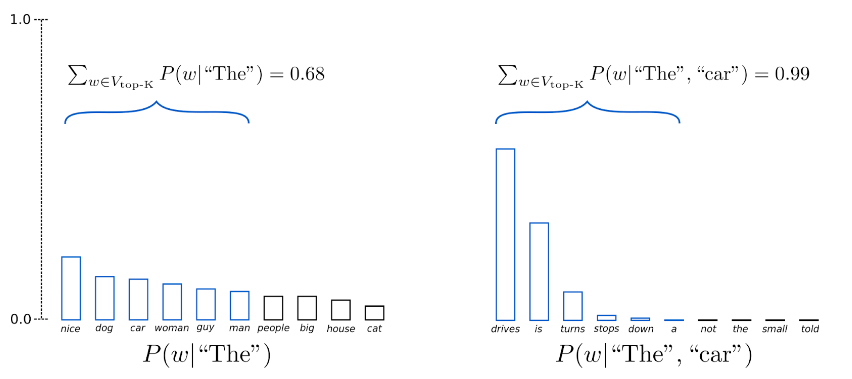
\includegraphics[width=0.9\linewidth]{figure/top_k.png}
\end{center}

\citebutton{huggingface, Patrick von Platen}{https://huggingface.co/blog/how-to-generate}

\end{vbframe}

% ------------------------------------------------------------------------------

\begin{vbframe}{Top-$k$ sampling}

\vfill

\textbf{Prompt: "Once upon a time"}
\begin{itemize}
    \item Top-$k$ , $k = 100$: \textit{"when I was young the internet was a mysterious landscape full of new and exciting ideas. I read ebooks, watched videos, read short stories"}
\end{itemize}
\vspace{2ex}

The quality has improved, but the fixed $k$ might be counterproductive\\
\vspace{2ex}
$\Rightarrow$ Make $k$ dynamic        


\end{vbframe}

% ------------------------------------------------------------------------------

\begin{vbframe}{Top-$p$ (Nucleus) sampling \citebutton{H\MakeLowercase{oltzman et al., 2019}}{\MakeLowercase{https://arxiv.org/abs/1904.09751}}}


Top-$p$ sampling chooses from the smallest possible set of tokens whose cumulative probability exceeds the probability threshold $p$. The probability mass is then redistributed accordingly.
Visualization with a threshold $p$ = 0.92:

\begin{center}
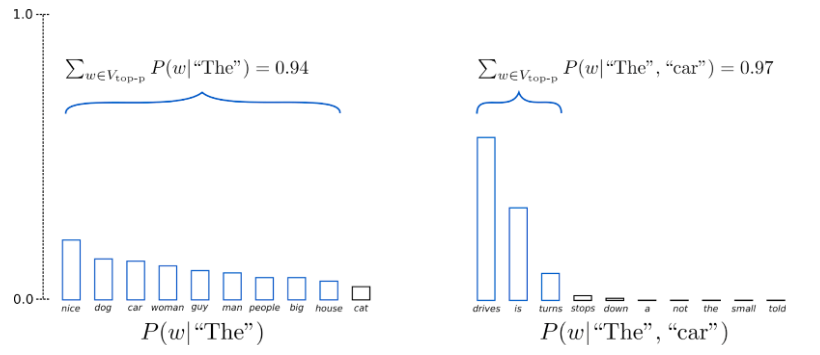
\includegraphics[width=1.0\linewidth]{figure/nucleus.png}
\end{center}

\citebutton{huggingface, Patrick von Platen}{https://huggingface.co/blog/how-to-generate}
\end{vbframe}

% ------------------------------------------------------------------------------

\begin{vbframe}{Top-$p$ (Nucleus) sampling}

\vfill
\textbf{Prompt: "Once upon a time"}
\begin{itemize}
    \item Top-$p$ , $p = 0.92$: \textit{"there were four major political parties in the United States. Since then, however, they have become even more of a novelty. For the past few decades, there have been only two."}
\end{itemize}

\vspace{2ex}

SOTA for many years, default decoding strategy in various GPT versions, but sometimes erratic depending on $p$ and the sampled tokens.\\

\vspace{2ex}

\textbf{Question:} Can there be a balance of coherence and diversity?\\
$\Rightarrow$ Contrastive search
  
\end{vbframe}

% ------------------------------------------------------------------------------

\begin{frame}{Contrastive Search \citebutton{S\MakeLowercase{u et al., 2022}}{\MakeLowercase{https://arxiv.org/abs/2210.14140}}}

\begin{center}
    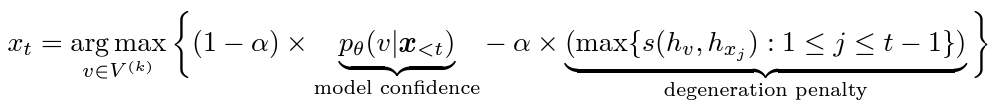
\includegraphics[width=1.0\linewidth]{figure/contrastive_search.png}
\end{center}     

When generating output, contrastive search jointly considers:
\begin{itemize}
    \item The probability predicted by the language model to maintain the semantic coherence between the generated text and the prompt.
    \item The similarity with respect to the previous context to avoid  degeneration (as in Greedy or Beam search)
\end{itemize}
   
$\Rightarrow$ An "ideal" token should have a high probability and bring diversity to the story.

Empirical studies suggest $k \in \{5, 8, 10, 15\}$ and $\alpha \in \{0.4, 0.5, 0.6\}$ \citebutton{Su \& Collier, 2023}{https://arxiv.org/abs/2210.14140} \citebutton{Su \& Xu, 2022}{https://arxiv.org/abs/2211.10797} \citebutton{Su et al., 2022}{https://arxiv.org/abs/2202.06417}

\vfill

\end{frame}

% ------------------------------------------------------------------------------

\begin{vbframe}{Contrastive Search formula}

\citebutton{huggingface, Tian Lan}{https://huggingface.co/blog/introducing-csearch}

\hspace{}

\textit{Let's have a closer look at the formula for Contrastive Search:}
\small
$$x_t = \underset{v \in V^{(k)}}{argmax}\left\{(1 - \alpha) \times \textcolor{red}{p_\theta(v|\mathbf{x}_{<t})} - \alpha \times \textcolor{blue}{(max\{s(h_v,h_{x_j}):1\leq j \leq t-1\})}\right\}$$

\begin{itemize}
    \item $x_t$ is the output token and $\mathbf{x}_{<t}$ the context
    \item $V^{(k)}$ is the set of top-k predictions from the models probability distribution (this is the same $k$ as in the top-$k$ sampling from earlier)
    \item $\textcolor{red}{p_\theta(v|\mathbf{x}_{<t})}$, the \textit{model confidence}, is the probability of a candidate token $v$ given the context
    \item $\textcolor{blue}{max\{s(h_v,h_{x_j}):1\leq j \leq t-1\}}$, the \textit{degeneration penalty}, measures how similar $v$ is to the context, $s()$ is the cosine similarity between the token representations
    \item The degeneration penalty is defined as the maximum cosine similarity between the token representation of $v$, i.e $h_v$, and of all tokens in the context $\mathbf{x}_{<t}$
    \item $h_v$ is computed by the language model given the concatination of $v$ and $\mathbf{x}_{<t}$
    \item In order to maximize the formula we want $v$ to have a high probability and a low degeneration penalty
    \item Intuitively, a larger degeneration penalty of $v$ means it is more similar (in the representation space) to the context, therefore more likely leading to the problem of model degeneration
    \item $\alpha$ determines how much weight to give to each component
    \item For $\alpha = 0$ we only consider the probability and contrastive search becomes greedy search
\end{itemize}

\vfill

\end{vbframe}

% ------------------------------------------------------------------------------

\begin{frame}{Contrastive Decoding \citebutton{L\MakeLowercase{i et al., 2023}}{\MakeLowercase{https://arxiv.org/abs/2210.15097}}}

\centering
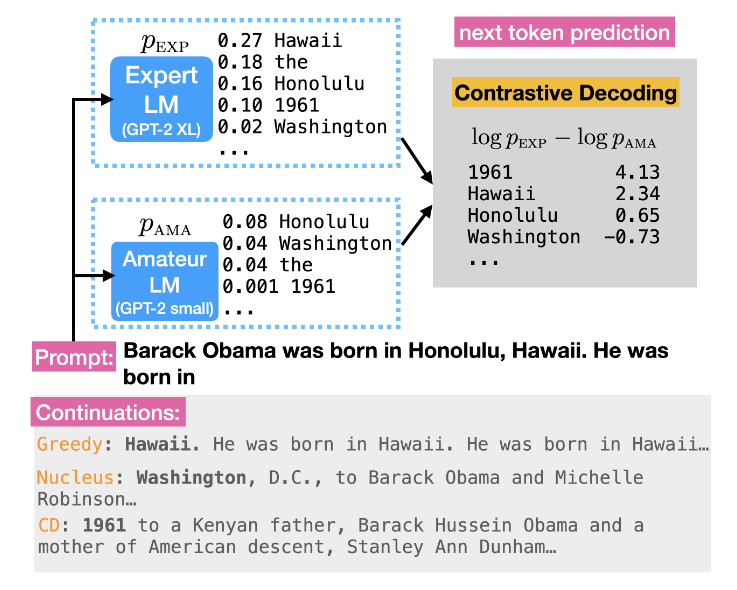
\includegraphics[width=0.7\textwidth]{chapters/chapter12/figure/cd.png}

\begin{itemize}
    \item Contrastive decoding exploits the contrasts
between expert and amateur LM of different sizes by
choosing tokens that maximize their log-likelihood
difference (read the paper if you are interested, not going into more detail here!)
\end{itemize}


\end{frame}

% ------------------------------------------------------------------------------

\endlecture
\end{document}